\documentclass{article}

\usepackage{amsmath, amsthm, amssymb, amsfonts}
\usepackage{thmtools}
\usepackage{graphicx}
\usepackage{setspace}
\usepackage{geometry}
\usepackage{float}
\usepackage{hyperref}
\usepackage[utf8]{inputenc}
\usepackage[english]{babel}
\usepackage{framed}
\usepackage[dvipsnames]{xcolor}
\usepackage{tcolorbox}
\usepackage{listings}


% Definición de colores y estilo para el código
\definecolor{codegreen}{rgb}{0,0.6,0}
\definecolor{codegray}{rgb}{0.5,0.5,0.5}
\definecolor{codepurple}{rgb}{0.58,0,0.82}
\definecolor{backcolour}{rgb}{0.95,0.95,0.92}
\lstdefinestyle{mystyle}{
    backgroundcolor=\color{backcolour},   
    commentstyle=\color{codegreen},
    keywordstyle=\color{magenta},
    numberstyle=\tiny\color{codegray},
    stringstyle=\color{codepurple},
    basicstyle=\ttfamily\footnotesize,
    breakatwhitespace=false,         
    breaklines=true,                 
    captionpos=b,                    
    keepspaces=true,                 
    %numbers=left,                    
    %numbersep=5pt,                  
    showspaces=false,                
    showstringspaces=false,
    showtabs=false,                  
    tabsize=2,
    literate={á}{{\'a}}1 {é}{{\'e}}1 {í}{{\'i}}1 {ó}{{\'o}}1 {ú}{{\'u}}1
}
\lstset{style=mystyle}

\colorlet{LightGray}{White!90!Periwinkle}
\colorlet{LightOrange}{Orange!15}
\colorlet{LightGreen}{Green!15}

\newcommand{\HRule}[1]{\rule{\linewidth}{#1}}

\declaretheoremstyle[name=Theorem,]{thmsty}
\declaretheorem[style=thmsty,numberwithin=section]{theorem}
\tcolorboxenvironment{theorem}{colback=LightGray}

\declaretheoremstyle[name=Proposition,]{prosty}
\declaretheorem[style=prosty,numberlike=theorem]{proposition}
\tcolorboxenvironment{proposition}{colback=LightOrange}

\declaretheoremstyle[name=Principle,]{prcpsty}
\declaretheorem[style=prcpsty,numberlike=theorem]{principle}
\tcolorboxenvironment{principle}{colback=LightGreen}

\setstretch{1.2}
\geometry{
    textheight=9in,
    textwidth=5.5in,
    top=1in,
    headheight=12pt,
    headsep=25pt,
    footskip=30pt
}

% ------------------------------------------------------------------------------

\begin{document}

% ------------------------------------------------------------------------------
% Cover Page and ToC
% ------------------------------------------------------------------------------

\title{ \normalsize \textsc{}
		\\ [2.0cm]
		\HRule{1.5pt} \\
		\LARGE \textbf{\uppercase{Tarea 12 - Metodos numericos}
		\HRule{2.0pt} \\ [0.6cm] \LARGE{} \vspace*{10\baselineskip}}
		}
\date{}
\author{\textbf{Guillermo Segura Gómez} \\ 
		Centro de Investigación en Matemáticas \\
		Métodos Numéricos \\
		  12 de noviembre de 2023}

\maketitle
\newpage


\section{Introducción}

Existen dos problemas fundamentales a resolver en las técnicas de aproximación. El primer problema es la aproximación de una función. Durante las tareas pasadas revisamos las técnicas de interpolación. La interpolación busca una aproximación a una función que pase por todos los puntos de la función. El segundo problema a resolver es el de ajustar funciones a un conjunto de datos establecidos, es decir, encontrar la mejor función para representar a los datos. Esto se conoce como \textbf{regresión} \cite{burden2015numerical}. Una de las mejores técnicas es el método de mínimos cuadrados. Este método consiste en minimizar una cantidad conocida como \textit{error cuadrático medio}. El problema general de mínimos cuadrados se puede resducir mediante una serie de cálculos a un problema de álgebra de matrices \cite{abdi2003partial}. Durante este trabajo revisaremos la técnica de mínimos cuadrados regularizados, una técnica de regresión la cual introduce un factor externo a los datos para evitar el sobre ajuste del modelo generado. 

Una aplicación de técnicas de interpolación es que se pueden utilizar para calcular integrales numéricamente, ya que las funciones interpoladas (generalmente polinomios) son funciones suaves y bien comportadas, las cuales funcionan bastante bien en los métodos de integración numérica. El método básico asociado con la aproximación de una integral se conoce como \textbf{cuadratura numérica}, el cual utiliza la sumas de coeficientes de polinomios para calcular las integrales. Durante este trabajo revisaremos las formulaciones de Newton Cortés abiertas y cerradas, las cuales son técnicas para integrar numéricamente que consisten en dividir un intervalo de integración en intervalos equidistantes. Además revisaremos la técnica de cuadratura gaussiana la cual no necesariamente divide el intervalo en sub intervalos equidistantes. 


\section{Problema 1}
Programar en C las técnicas de derivación para la primera (derivación hacia adelante, hacia atrás, centrada, 3 puntos, 5 puntos vistos en clase) y segunda derivada (fórmula del punto medio visto en clase) de una función arbitraria. Utilizando la siguiente tabla y las fórmulas programadas, aproxima adecuadamente $f^{\prime}(1,3)$ y $f^{\prime \prime}(1,3)$, con $h=0.1,0.01$, según corresponda y compara con los verdaderos valores si $f(x)=3 x e^x-\cos (x)$,
\begin{tabular}{l|l|l|l|l|l}
$x$ & 1.20 & 1.29 & 1.30 & 1.31 & 1.40 \\
\hline$f(x)$ & 11.59006 & 13.78176 & 14.04276 & 14.30741 & 16.86187
\end{tabular}

Encontrar los valores $\lambda_i$ es todo un problema de optimización, para nuestro fines consideremos que los valores son constantes, es decir, $\lambda=\lambda_i, \forall i$.

\subsection{Pseudocódigo}

El problema de mínimos cuadrados se puede mejorar mediante la introducción de información adicional para solucionar un problema mal definido o para evitar sobreajuste. Se introduce un término $\lambda$ que regulariza la importancia de ciertos datos y así tener soluciones mas generales y menos sobreajustadas. 
El sistema a resolver para mínimos cuadrados regularizados queda de la forma

\begin{equation}
    (\Phi^T \Phi + \alpha)c = \Phi^T y
\end{equation}

en donde $\Phi$ es la matriz de las funciones base sobre las cuales se esta realizando el ajuste. 
Para la implementación el funcionamiento del programa en sus pasos mas fundamentales es el siguiente:
\begin{enumerate}
    \item Se construye la matriz $\Phi$
    \item Se construye el sistema $Ac = b$. En donde $A = \Phi^T \Phi + \alpha$ y $b = \Phi^T y$
    \item Se resuelve el sistema $Ac = b$ mediante un método numérico.
\end{enumerate}

La lógica en la construcción de la matriz $\Phi$ es prácticamente la misma en los tres casos. Se presenta el pseudocódigo de la función polinomial.

\begin{lstlisting}[language=C, caption={Construcción de la matriz Phi para ajuste polinomial.}]
void MatrixBuild(double* Phi, int rows, int cols, double* x, int n) {
  // Para cada observación
  for (int i = 0; i < rows; i++) { 
    // Término constante, x^0
    Phi[i * cols] = 1.0;
    // Para cada término del polinomio
    for (int j = 1; j < cols; j++) { 
      // x^j para la observación i
      Phi[i * cols + j] = pow(x[i], j); 
    }
  }
}
\end{lstlisting}

A continuación se presenta el pseudocódigo para la función que construye el sistema $Ac = b$.

\begin{lstlisting}[language=Pascal, caption={Pseudocódigo de la función buildSystem.}]
Función buildSystem(m: Entero, n: Entero, x: Arreglo de Real, y: Arreglo de Real, A: Arreglo de Real, b: Arreglo de Real, lambda: Real, option: Entero)

    // Reservar memoria para la matriz Phi de size n*m
    Phi := ReservarMemoria(n * m)
    Si Phi es NULL entonces
        MostrarError("Error al asignar memoria.")
        TerminarEjecución()
    FinSi

    // Construir la matriz Phi basada en la opción seleccionada
    Según option hacer
        caso 1:
            MatrixBuild(Phi, n, m, x, n)
        caso 2:
            MatrixBuildTrig(Phi, n, m, x, n)
        caso 3:
            MatrixBuildRBF(Phi, n, m, x)
        caso contrario:
            MostrarError("Ajuste no reconocido")
            TerminarEjecución()
    FinSegún

    // Reservar memoria para la matriz transpuesta PhiT de size m*n
    PhiT := ReservarMemoria(n * m)
    Si PhiT es NULL entonces
        MostrarError("Error al asignar memoria para PhiT.")
        LiberarMemoria(Phi)
        TerminarEjecución()
    FinSi

    // Transponer la matriz Phi y almacenar en PhiT
    MatrixT(n, m, Phi, PhiT)

    // Reservar memoria para la matriz Alpha de size m*m e inicializar en cero
    Alpha := ReservarCeroMemoria(m * m)
    Si Alpha es NULL entonces
        MostrarError("Error al asignar memoria para Alpha.")
        LiberarMemoria(Phi)
        LiberarMemoria(PhiT)
        TerminarEjecución()
    FinSi

    // Asignar lambda en la diagonal de la matriz Alpha
    Para i := 0 hasta m-1 hacer
        Alpha[i * m + i] := lambda
    FinPara

    // Reservar memoria para PhiProd que es el producto de PhiT * Phi
    PhiProd := ReservarMemoria(m * m)

    // Calcular el producto de matrices PhiT y Phi y almacenar en PhiProd
    MatrixProduct(PhiT, Phi, PhiProd, m, n, m)
    MatrixSum(PhiProd, Alpha, A, m, m)

    // Construir b como el producto de PhiT y y
    Si b es NULL entonces
        MostrarError("Error al asignar memoria para b.")
        LiberarMemoria(Phi)
        LiberarMemoria(PhiT)
        LiberarMemoria(Alpha)
        LiberarMemoria(A)
        LiberarMemoria(PhiProd)
        TerminarEjecución()
    FinSi
    MatrixProduct(PhiT, y, b, m, n, 1)

    // Liberar memoria utilizada por la función
    LiberarMemoria(Phi)
    LiberarMemoria(PhiT)
    LiberarMemoria(Alpha)
    LiberarMemoria(PhiProd)

FinFunción
\end{lstlisting}

\subsection{Ejecución}

El código con nombre \textbf{Minimus2coeff.c} regresa el valor de los coeficientes utilizando los tres enfoques, polinomial, trigonométrico y radial. Para datos del libro burden tenemos el siguiente resultado \cite{burden2015numerical}.

\begin{lstlisting}
guillermo_sego@192 Tarea11 % make
gcc -g -o build/Debug/Minimus2coeff.o -c Minimus2coeff.c
gcc -g -o build/Minimus2coeff build/Debug/matrix.o build/Debug/Minimus2coeff.o
guillermo_sego@192 Tarea11 % ./build/Minimus2coeff
Los coeficientes del ajuste m = 2 para opción polinómica son los siguientes:
-0.360000 
1.538182 
Los coeficientes del ajuste m = 2 para opción trigonométrica son los siguientes:
7.785868 
-1.683429 
Los coeficientes del ajuste m = 2 para opción radial son los siguientes:
-0.876910 
4.930649 
\end{lstlisting}

Se comparan con el ejemplo 8.1 y los coeficientes del ajuste polinomial son los mismos. 

Probamos los códigos para datos del libro burden y tenemos lo siguiente.

\section{Problema 2}
Para evaluar los códigos del ejercicio 1 . Consideremos la función de Sutherland que define la viscosidad de un gas según la temperatura $T$ en Kelvin (entre 1000), definida por $f(x)=m_0\left(\frac{1000 T}{T_0}\right)^{\frac{3}{2}}\left(\frac{T_0+S_u}{1000 T+S_u}\right)$. Calculemos la viscosidad del oxígeno $O_2$, para ello usemos $m_0=1.919 e^{-2}, T_0=273$, y $S_u=139$. Realiza lo siguiente:

a) Evalúa los puntos $T i=[0.273,0.303,0.323,0.353,0.423,0.573,1.473]$ en la función de Sutherland. Los puntos $T i$ corresponden a los $n+1$ puntos $x i$, y las evaluaciones son los valores yi (estamos simulando que se ha realizado un experimento de laboratorio físico, es decir, sólo tenemos mediciones experimentales).

b) Usando el valor de $\lambda$ = 0, 1e-5, 1e-7, para 0 $\leq$ i $\leq$ n, aplica las 3 funciones de interpolación programadas obtenidas del método de mínimos cuadrados en el inciso 1), con ellos calcula la viscosidad para T = 1.2, compara con el valor real obtenido directamente con la función de Sutherland.

c) Gráfica las soluciones obtenidas en el intervalo [0.273, 1.5], usa incrementos de =0.05. 

d) Repite los incisos a), b) y c), pero con los nodos T i = [0.273, 0.473, 0.673, 0.873, 0.1073, 0.1273, 1.473].

¿Qué puedes concluir de los nodos y el comportamiento de las funciones de interpolación según $\lambda$?


Las funciones son las mismas utilizadas en el problema anterior.

\subsection{Ejecución}
Para la ejecución y evaluación de un punto $T$ en los polinomios calculados se utilizó el código \textbf{Minimus2c}. Para la evaluación se generaron funciones para cada caso. Todo vive en la biblioteca \textbf{matrix.h}.

Se escoje la opción de ajuste que se va realizar. Esta fue la razón por la cual se construyeron de esta manera las funciones. Se construyeron lo mas general posible para poder tener este tipo de espacio de trabajo sobre los cuales evaluar y comparar los resultados sin hacer cambios al programa utilizando los tres tipos de ajuste.

Para el polinomial
\begin{lstlisting}
guillermo_sego@192 Tarea11 % make                 
gcc -g -o build/Debug/Minimus2n.o -c Minimus2n.c
gcc -g -o build/Minimus2n build/Debug/matrix.o build/Debug/Minimus2n.o
guillermo_sego@192 Tarea11 % ./build/Minimus2n    
Introduce el tipo de ajuste:
1. Polinomial
2. Trigonométrico
3. Radial
1
Tabla de Evaluaciones para T = 1.2
m \ lambda      0.000000e+00    1.000000e-05    1.000000e-07
2               0.052802        0.052802        0.052802
3               0.055654        0.055650        0.055654
4               0.057924        0.057921        0.057924
5               0.061330        0.061328        0.061330

El valor real de la función de Sutherland para T = 1.2 es: 0.054415
\end{lstlisting}

Para el trigonométrico
\begin{lstlisting}
guillermo_sego@192 Tarea11 % ./build/Minimus2n
Introduce el tipo de ajuste:
1. Polinomial
2. Trigonométrico
3. Radial
2
Tabla de Evaluaciones para T = 1.2
m \ lambda      0.000000e+00    1.000000e-05    1.000000e-07
2               -0.007621       -0.007608       -0.007621
3               0.003425        0.003425        0.003425
4               0.001637        0.001653        0.001637
5               -0.011584       -0.011575       -0.011584

El valor real de la función de Sutherland para T = 1.2 es: 0.054415
\end{lstlisting}

Para el radial
\begin{lstlisting}
guillermo_sego@192 Tarea11 % ./build/Minimus2n
Introduce el tipo de ajuste:
1. Polinomial
2. Trigonométrico
3. Radial
3
Tabla de Evaluaciones para T = 1.2
m \ lambda      0.000000e+00    1.000000e-05    1.000000e-07
2               0.488342        0.469090        0.488141
3               0.624499        0.615662        0.624410
4               0.660465        0.657121        0.660432
5               0.509973        0.509386        0.509967

El valor real de la función de Sutherland para T = 1.2 es: 0.054415
\end{lstlisting}

Es evidente que el ajuste que mejor se aproxima a la función es el polinómico. 
Se graficaron los resultados para diferentes valores de $m$ y también diferentes valores de lambda. En la figura \ref{m} tenemos diferentes valores de m. Luego vemos los diferentes valores de lambda en la figura \ref{lambda}.

Repitiendo el proceso para el caso del inciso d. 

Para el polinomial
\begin{lstlisting}
guillermo_sego@192 Tarea11 % ./build/Minimus2n
Introduce el tipo de ajuste:
1. Polinomial
2. Trigonométrico
3. Radial
1
Tabla de Evaluaciones para T = 1.2
m \ lambda      0.000000e+00    1.000000e-05    1.000000e-07
2               0.054778        0.054778        0.054778
3               0.055588        0.055587        0.055588
4               0.053717        0.053736        0.053717
5               0.052658        0.052668        0.052658

El valor real de la función de Sutherland para T = 1.2 es: 0.054415
\end{lstlisting}

Para el trigonométrico
\begin{lstlisting}
guillermo_sego@192 Tarea11 % ./build/Minimus2n
Introduce el tipo de ajuste:
1. Polinomial
2. Trigonométrico
3. Radial
2
Tabla de Evaluaciones para T = 1.2
m \ lambda      0.000000e+00    1.000000e-05    1.000000e-07
2               -0.017440       -0.017425       -0.017440
3               0.102610        0.088996        0.102454
4               -0.004737       -0.004739       -0.004737
5               -0.017345       -0.017344       -0.017345

El valor real de la función de Sutherland para T = 1.2 es: 0.054415
\end{lstlisting}

Para el radial
\begin{lstlisting}
guillermo_sego@192 Tarea11 % ./build/Minimus2n
Introduce el tipo de ajuste:
1. Polinomial
2. Trigonométrico
3. Radial
3
Tabla de Evaluaciones para T = 1.2
m \ lambda      0.000000e+00    1.000000e-05    1.000000e-07
2               0.070989        0.070978        0.070989
3               0.125816        0.124826        0.125806
4               0.133624        0.133498        0.133623
5               0.245382        0.245092        0.245379

El valor real de la función de Sutherland para T = 1.2 es: 0.054415
\end{lstlisting}

Graficamos para diferentes valores de lambda en este caso. Vemos la gráfica en la figura \ref{lambdad}.

Es evidente que hay algo incorrecto en las funcione generadoras para los caos trigonométrico y radial. La conclusión que podemos determinar en base a la correcta aproximación polinomial para lambda es que en función de este valor podemos introducir correcciones para evitar el sobre ajuste, es decir, cuando tenemos un modelo que esta sobre ajustado, un nuevo conjunto de datos del mismo experimento no se puede determinar. Los valores de lambda permiten generalizar el modelo y asi tener predicciones mas precisas para los nuevos conjuntos de datos. 

\section{Problema 3}
Crea una librería en $\mathrm{C}$ que calcule la aproximación a una integral en el intervalo [a,b] arbitrario con los métodos de Newton-Cotes abierto $(\mathrm{n}=0,1,2,3)$, Newton-Cotes cerrado $(\mathrm{n}=1,2,3,4)$, y cuadratura gaussiana $(\mathrm{n}=1,2,3,4,5)$. Con las librerías aproxima las siguientes integrales:
\begin{equation*}
    \int_0^{\pi / 4} \sin (x) d x, \quad \int_1^{1,5} x^2 \ln x d x, \quad \int_0^1 x^2 e^{-x} d x
\end{equation*}
NOTA: Crea una tabla comparativa de los resultados. OJO: La primer integral es la vista en clase.

Se construyó la librería en el archivo \textbf{integration.c}. 

\subsection{Pseudocódigo}
Los códigos tienen estructura similar debido a que se utilizan fórmulas. Sólo se presenta el pseudocódigo de la primer función.

\begin{lstlisting}[language=Pascal, caption={Newton-Cotes Abierto de orden 0 (Punto Medio)}]
function NewtonCotesAbiertoOrdenCero(a: real; b: real; f: function): real;
var
    h: real;
    puntoMedio: real;
    resultado: real;
begin
    h := b - a;
    puntoMedio := a + h / 2.0;
    resultado := h * f(puntoMedio);
    return resultado;
end;
\end{lstlisting}


\subsection{Ejecución}
Vamos a evaluar las integrales y compararlas en un solo programa. A continuación se presenta la ejecución del código.

\begin{lstlisting}
    guillermo_sego@192 Tarea11 % make
gcc -g -o build/Debug/IntegralExamples.o -c IntegralExamples.c
gcc -g -o build/IntegralExamples build/Debug/integration.o build/Debug/IntegralExamples.o
guillermo_sego@192 Tarea11 % ./build/IntegralExamples
Method                  | Integral of sin(x)    | Integral of x^2 * ln(x) | Integral of x^2 * e^(-x)
-----------------|----------------|------------------|--------------
NC Open Order 0         | 0.3005588649            | 0.1743308995               | 0.1516326649
NC Open Order 1         | 0.2979875422            | 0.1803127496               | 0.1538999882
NC Open Order 2         | 0.2928586592            | 0.1922716135               | 0.1590432683
NC Open Order 3         | 0.2928692281            | 0.1922678867               | 0.1595142015
NC Closed Order 1       | 0.2776801836            | 0.2280741233               | 0.1839397206
NC Closed Order 2       | 0.2929326378            | 0.1922453074               | 0.1624016835
NC Closed Order 3       | 0.2929107025            | 0.1922530931               | 0.1614099213
NC Closed Order 4       | 0.2928931826            | 0.1922593373               | 0.1606105287
Gauss Quadrature Order 1| 0.3005588649            | 0.1743308995               | 0.1516326649
Gauss Quadrature Order 2| 0.2928669073            | 0.1922687064               | 0.1594104310
Gauss Quadrature Order 3| 0.2928932536            | 0.1922593773               | 0.1605953868
Gauss Quadrature Order 4| 0.2928932188            | 0.1922593578               | 0.1606027775
Gauss Quadrature Order 5| 0.3403824597            | 0.2353897363               | 0.1978182805
\end{lstlisting}

\section{Problema 4}


Investiga el método de extrapolación Richardson, y el método de Romberg, presenta un ejemplo. 

\subsection{Métodos de Extrapolación de Richardson y Método de Romberg}

La búsqueda de precisión en el cálculo numérico de integrales ha llevado al desarrollo de métodos sofisticados que mejoran las estimaciones aproximadas. Entre estas técnicas, la extrapolación de Richardson y el método de Romberg se destacan por su capacidad para refinar sucesivamente las aproximaciones. \cite{burden2015numerical}

\subsection{Extrapolación de Richardson}

El método de extrapolación de Richardson aprovecha la relación entre el tamaño del paso de una aproximación numérica y su error asociado. Este procedimiento se basa en el cálculo de dos aproximaciones sucesivas, con tamaños de paso diferentes, para extrapolar una aproximación que sería obtenida con un paso hipotéticamente igual a cero, donde el error es mínimo. 

El fundamento de este método reside en la suposición de que el error se comporta de manera polinomial respecto al tamaño del paso. Con dos estimaciones, \( f(h) \) y \( f(h/2) \), se puede eliminar el término principal del error y obtener una aproximación mejorada. Esta técnica es particularmente eficiente cuando se combina con métodos de alta precisión para la integración numérica. \cite{burden2015numerical}

\subsection{Método de Romberg}

El método de Romberg es una aplicación específica de la extrapolación de Richardson en la integración numérica. Se basa en la Regla del Trapecio y utiliza una secuencia de aproximaciones de la integral con tamaños de paso decrecientes, que son halved sucesivamente. Aplicando la extrapolación de Richardson a estas aproximaciones, Romberg construye una tabla de extrapolación, donde cada nivel sucesivo aumenta el orden de precisión de la aproximación. La convergencia es generalmente rápida, y el resultado tiende a ser muy preciso. \cite{burden2015numerical}

\subsection{Ejemplo de Aplicación}

Consideremos la integral definida $\int_{0}^{1} e^{-x^2} dx )$, cuyo valor exacto no es sencillo calcular simbólicamente. Utilizando la Regla del Trapecio con un solo intervalo, obtenemos una primera aproximación. Repitiendo con dos intervalos, y luego aplicando la extrapolación de Richardson, se mejora la estimación. Continuando este proceso, y aplicando el método de Romberg, se construye una tabla de valores que converge rápidamente al valor exacto de la integral.

\begin{figure}
    \centering
    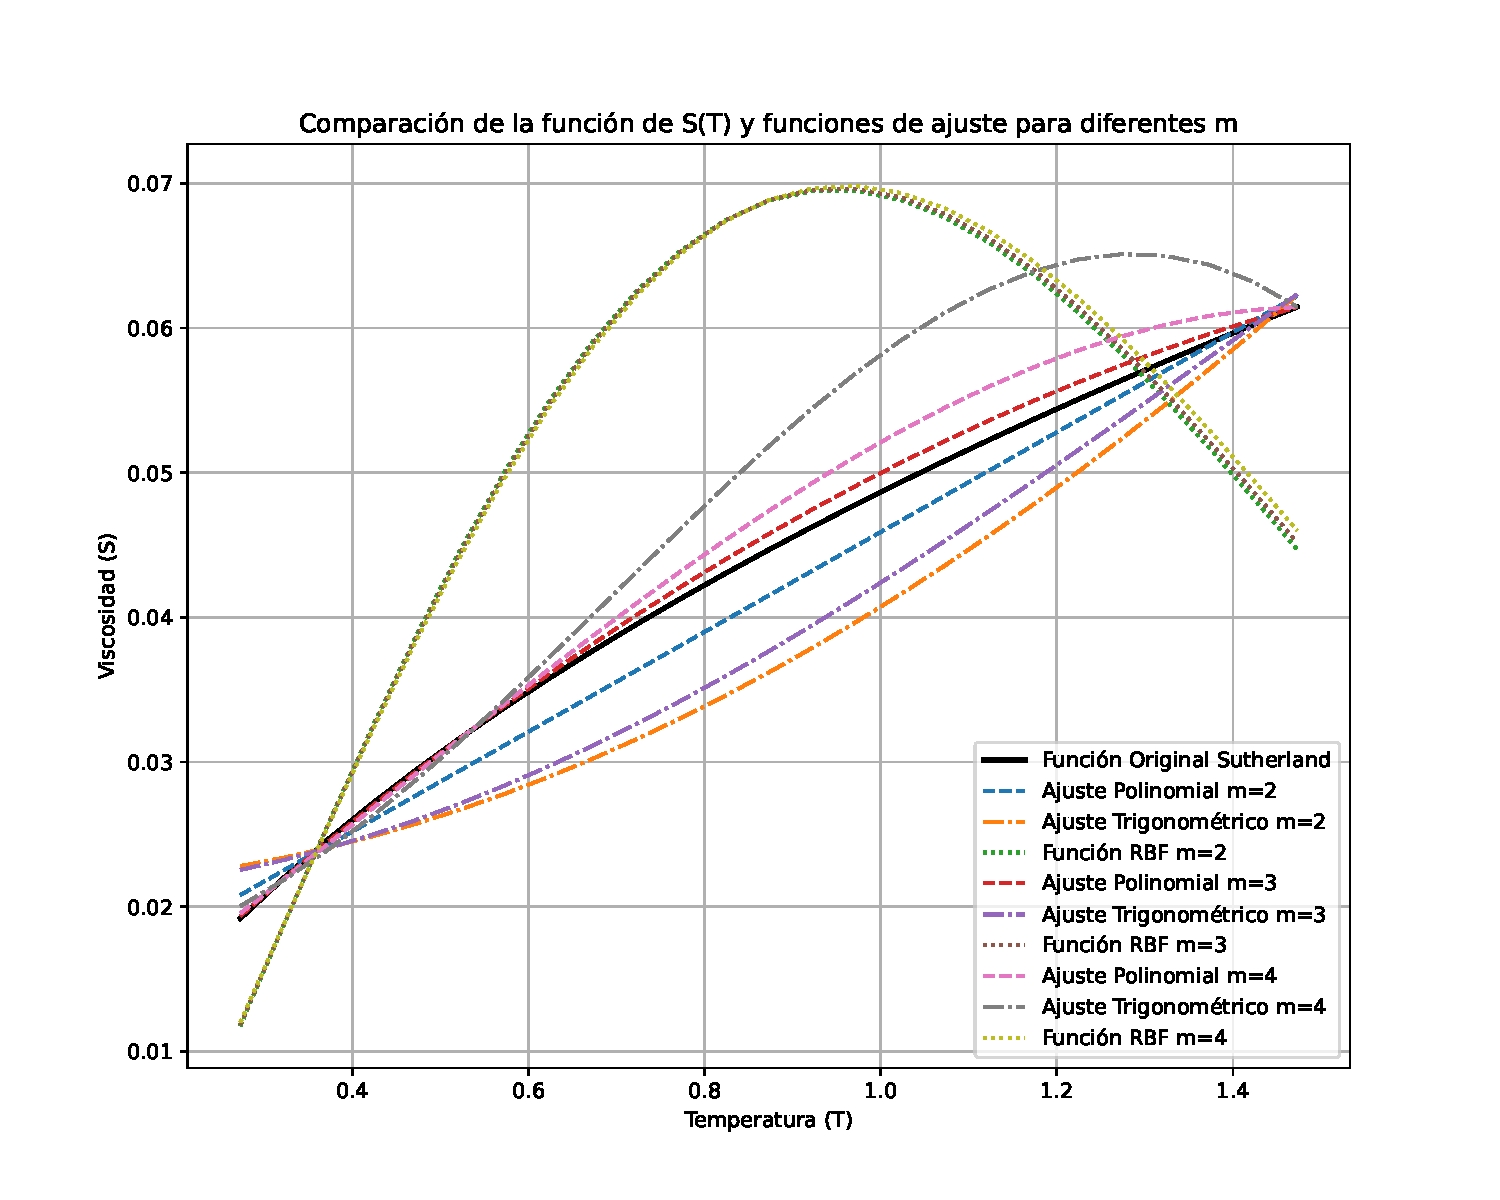
\includegraphics[scale=0.5]{comparacion_ajustes.pdf}
    \caption{Comparación curvas de ajuste para diferentes valores de lambda para el inciso d}
    \label{lambdad}
\end{figure}


\section{Conclusión}
Durante este trabajo realizamos un estudio acerca de las técnicas de aproximación, el problema de aproximación a un conjunto de datos (mínimos cuadrados) y una aplicación de la aproximación de funciones por polinomios en la integración numérica. El problema general de mínimos cuadrados resulta de la solución de un sistema matricial. El término que añadimos para evitar sobre ajuste nos permite tener un mejor modelo, mas general y mejor adaptado a los diferentes conjuntos de datos. Además las aproximaciones a funciones, nos permite integrar numéricamente funciones cuyas integrales pueden ser muy complicadas o directamente no existen. En general las aproximaciones difieren muy poco cuando cambiamos el orden. Para términos prácticos en los que no necesitamos tanta precisión es indistinguible el método de integración. Para cuestiones en las que si se necesite algo muy específico necesitamos evaluar la precisión de las aproximaciones. 

\bibliographystyle{IEEEtran}
\bibliography{ref.bib}

\end{document}
